\documentclass{book}
\usepackage[a4paper,top=2.5cm,bottom=2.5cm,left=2.5cm,right=2.5cm]{geometry}
\usepackage{makeidx}
\usepackage{natbib}
\usepackage{graphicx}
\usepackage{multicol}
\usepackage{float}
\usepackage{listings}
\usepackage{color}
\usepackage{ifthen}
\usepackage[table]{xcolor}
\usepackage{textcomp}
\usepackage{alltt}
\usepackage{ifpdf}
\ifpdf
\usepackage[pdftex,
            pagebackref=true,
            colorlinks=true,
            linkcolor=blue,
            unicode
           ]{hyperref}
\else
\usepackage[ps2pdf,
            pagebackref=true,
            colorlinks=true,
            linkcolor=blue,
            unicode
           ]{hyperref}
\usepackage{pspicture}
\fi
\usepackage[utf8]{inputenc}
\usepackage{mathptmx}
\usepackage[scaled=.90]{helvet}
\usepackage{courier}
\usepackage{sectsty}
\usepackage{amssymb}
\usepackage[titles]{tocloft}
\usepackage{doxygen}
\lstset{language=C++,inputencoding=utf8,basicstyle=\footnotesize,breaklines=true,breakatwhitespace=true,tabsize=8,numbers=left }
\makeindex
\setcounter{tocdepth}{3}
\renewcommand{\footrulewidth}{0.4pt}
\renewcommand{\familydefault}{\sfdefault}
\hfuzz=15pt
\setlength{\emergencystretch}{15pt}
\hbadness=750
\tolerance=750
\begin{document}
\hypersetup{pageanchor=false,citecolor=blue}
\begin{titlepage}
\vspace*{7cm}
\begin{center}
{\Large Libusb++ \\[1ex]\large 1.\-0 }\\
\vspace*{1cm}
{\large Generated by Doxygen 1.8.1.2}\\
\vspace*{0.5cm}
{\small Sat Sep 8 2012 17:02:56}\\
\end{center}
\end{titlepage}
\clearemptydoublepage
\pagenumbering{roman}
\tableofcontents
\clearemptydoublepage
\pagenumbering{arabic}
\hypersetup{pageanchor=true,citecolor=blue}
\chapter{Todo List}
\label{todo}
\hypertarget{todo}{}

\begin{DoxyRefList}
\item[\label{todo__todo000001}%
\hypertarget{todo__todo000001}{}%
Member \hyperlink{class_lib_u_s_b_1_1_lib_u_s_b_a532d474d390477dffd2109e8540be558}{Lib\-U\-S\-B\-:\-:Lib\-U\-S\-B\-:\-:Device\-Factory\-\_\-t} )(std\-::shared\-\_\-ptr$<$ Device\-Impl $>$)]Replace with std\-::function? 
\end{DoxyRefList}
\chapter{Class Index}
\section{Class Hierarchy}
This inheritance list is sorted roughly, but not completely, alphabetically\-:\begin{DoxyCompactList}
\item \contentsline{section}{Lib\-U\-S\-B\-:\-:Configuration}{\pageref{class_lib_u_s_b_1_1_configuration}}{}
\item \contentsline{section}{Lib\-U\-S\-B\-:\-:Device}{\pageref{class_lib_u_s_b_1_1_device}}{}
\item \contentsline{section}{Lib\-U\-S\-B\-:\-:Endpoint}{\pageref{class_lib_u_s_b_1_1_endpoint}}{}
\item \contentsline{section}{Lib\-U\-S\-B\-:\-:Interface}{\pageref{class_lib_u_s_b_1_1_interface}}{}
\item \contentsline{section}{Lib\-U\-S\-B\-:\-:Lib\-U\-S\-B}{\pageref{class_lib_u_s_b_1_1_lib_u_s_b}}{}
\item \contentsline{section}{Lib\-U\-S\-B\-:\-:Lib\-U\-S\-B\-Exception}{\pageref{class_lib_u_s_b_1_1_lib_u_s_b_exception}}{}
\item \contentsline{section}{Lib\-U\-S\-B\-:\-:Transfer}{\pageref{class_lib_u_s_b_1_1_transfer}}{}
\begin{DoxyCompactList}
\item \contentsline{section}{Lib\-U\-S\-B\-:\-:Bulk\-Transfer}{\pageref{class_lib_u_s_b_1_1_bulk_transfer}}{}
\item \contentsline{section}{Lib\-U\-S\-B\-:\-:Control\-Transfer}{\pageref{class_lib_u_s_b_1_1_control_transfer}}{}
\item \contentsline{section}{Lib\-U\-S\-B\-:\-:Interrupt\-Transfer}{\pageref{class_lib_u_s_b_1_1_interrupt_transfer}}{}
\item \contentsline{section}{Lib\-U\-S\-B\-:\-:Isochronous\-Transfer}{\pageref{class_lib_u_s_b_1_1_isochronous_transfer}}{}
\end{DoxyCompactList}
\end{DoxyCompactList}

\chapter{Class Index}
\section{Class List}
Here are the classes, structs, unions and interfaces with brief descriptions\-:\begin{DoxyCompactList}
\item\contentsline{section}{\hyperlink{class_lib_u_s_b_1_1_bulk_transfer}{Lib\-U\-S\-B\-::\-Bulk\-Transfer} \\*U\-S\-B Bulk \hyperlink{class_lib_u_s_b_1_1_transfer}{Transfer} object }{\pageref{class_lib_u_s_b_1_1_bulk_transfer}}{}
\item\contentsline{section}{\hyperlink{class_lib_u_s_b_1_1_configuration}{Lib\-U\-S\-B\-::\-Configuration} }{\pageref{class_lib_u_s_b_1_1_configuration}}{}
\item\contentsline{section}{\hyperlink{class_lib_u_s_b_1_1_control_transfer}{Lib\-U\-S\-B\-::\-Control\-Transfer} \\*U\-S\-B Control transfer object }{\pageref{class_lib_u_s_b_1_1_control_transfer}}{}
\item\contentsline{section}{\hyperlink{class_lib_u_s_b_1_1_device}{Lib\-U\-S\-B\-::\-Device} \\*Libusb device interface }{\pageref{class_lib_u_s_b_1_1_device}}{}
\item\contentsline{section}{\hyperlink{class_lib_u_s_b_1_1_endpoint}{Lib\-U\-S\-B\-::\-Endpoint} \\*U\-S\-B endpoint class }{\pageref{class_lib_u_s_b_1_1_endpoint}}{}
\item\contentsline{section}{\hyperlink{class_lib_u_s_b_1_1_interface}{Lib\-U\-S\-B\-::\-Interface} \\*U\-S\-B \hyperlink{class_lib_u_s_b_1_1_interface}{Interface} class }{\pageref{class_lib_u_s_b_1_1_interface}}{}
\item\contentsline{section}{\hyperlink{class_lib_u_s_b_1_1_interrupt_transfer}{Lib\-U\-S\-B\-::\-Interrupt\-Transfer} \\*U\-S\-B Interrupt \hyperlink{class_lib_u_s_b_1_1_transfer}{Transfer} object }{\pageref{class_lib_u_s_b_1_1_interrupt_transfer}}{}
\item\contentsline{section}{\hyperlink{class_lib_u_s_b_1_1_isochronous_transfer}{Lib\-U\-S\-B\-::\-Isochronous\-Transfer} \\*U\-S\-B Isochronous \hyperlink{class_lib_u_s_b_1_1_transfer}{Transfer} object }{\pageref{class_lib_u_s_b_1_1_isochronous_transfer}}{}
\item\contentsline{section}{\hyperlink{class_lib_u_s_b_1_1_lib_u_s_b}{Lib\-U\-S\-B\-::\-Lib\-U\-S\-B} \\*Contains static methods for enumerating devices }{\pageref{class_lib_u_s_b_1_1_lib_u_s_b}}{}
\item\contentsline{section}{\hyperlink{class_lib_u_s_b_1_1_lib_u_s_b_exception}{Lib\-U\-S\-B\-::\-Lib\-U\-S\-B\-Exception} }{\pageref{class_lib_u_s_b_1_1_lib_u_s_b_exception}}{}
\item\contentsline{section}{\hyperlink{class_lib_u_s_b_1_1_transfer}{Lib\-U\-S\-B\-::\-Transfer} \\*U\-S\-B Data transfer object }{\pageref{class_lib_u_s_b_1_1_transfer}}{}
\end{DoxyCompactList}

\chapter{Class Documentation}
\hypertarget{class_lib_u_s_b_1_1_bulk_transfer}{\section{Lib\-U\-S\-B\-:\-:Bulk\-Transfer Class Reference}
\label{class_lib_u_s_b_1_1_bulk_transfer}\index{Lib\-U\-S\-B\-::\-Bulk\-Transfer@{Lib\-U\-S\-B\-::\-Bulk\-Transfer}}
}


U\-S\-B Bulk \hyperlink{class_lib_u_s_b_1_1_transfer}{Transfer} object.  




{\ttfamily \#include $<$Transfer.\-h$>$}



Inheritance diagram for Lib\-U\-S\-B\-:\-:Bulk\-Transfer\-:\nopagebreak
\begin{figure}[H]
\begin{center}
\leavevmode
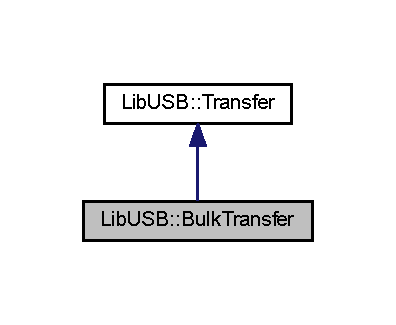
\includegraphics[width=190pt]{class_lib_u_s_b_1_1_bulk_transfer__inherit__graph}
\end{center}
\end{figure}


Collaboration diagram for Lib\-U\-S\-B\-:\-:Bulk\-Transfer\-:\nopagebreak
\begin{figure}[H]
\begin{center}
\leavevmode
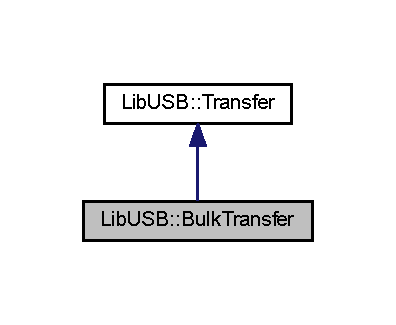
\includegraphics[width=190pt]{class_lib_u_s_b_1_1_bulk_transfer__coll__graph}
\end{center}
\end{figure}
\subsection*{Public Member Functions}
\begin{DoxyCompactItemize}
\item 
\hypertarget{class_lib_u_s_b_1_1_bulk_transfer_ac9e1f20fa379b49a0b7494bf2509d11f}{{\bfseries Bulk\-Transfer} (std\-::shared\-\_\-ptr$<$ Transfer\-Impl $>$ p\-Transfer\-Impl)}\label{class_lib_u_s_b_1_1_bulk_transfer_ac9e1f20fa379b49a0b7494bf2509d11f}

\end{DoxyCompactItemize}
\subsection*{Additional Inherited Members}


\subsection{Detailed Description}
U\-S\-B Bulk \hyperlink{class_lib_u_s_b_1_1_transfer}{Transfer} object. 

The documentation for this class was generated from the following file\-:\begin{DoxyCompactItemize}
\item 
headers/Transfer.\-h\end{DoxyCompactItemize}

\hypertarget{class_lib_u_s_b_1_1_configuration}{\section{Lib\-U\-S\-B\-:\-:Configuration Class Reference}
\label{class_lib_u_s_b_1_1_configuration}\index{Lib\-U\-S\-B\-::\-Configuration@{Lib\-U\-S\-B\-::\-Configuration}}
}
\subsection*{Public Member Functions}
\begin{DoxyCompactItemize}
\item 
\hypertarget{class_lib_u_s_b_1_1_configuration_a85966788f5f320aba04c98eae92f8512}{{\bfseries Configuration} (std\-::shared\-\_\-ptr$<$ Configuration\-Impl $>$ p\-Init)}\label{class_lib_u_s_b_1_1_configuration_a85966788f5f320aba04c98eae92f8512}

\item 
\hypertarget{class_lib_u_s_b_1_1_configuration_ae1dd391b9d615ff1fe80264585527dda}{std\-::wstring \hyperlink{class_lib_u_s_b_1_1_configuration_ae1dd391b9d615ff1fe80264585527dda}{Descriptor\-String} () const }\label{class_lib_u_s_b_1_1_configuration_ae1dd391b9d615ff1fe80264585527dda}

\begin{DoxyCompactList}\small\item\em Returns the string descriptor describing this configuration. \end{DoxyCompactList}\item 
\hypertarget{class_lib_u_s_b_1_1_configuration_af50cb780a19692834d7c1c107602c24c}{uint8\-\_\-t \hyperlink{class_lib_u_s_b_1_1_configuration_af50cb780a19692834d7c1c107602c24c}{Value} () const }\label{class_lib_u_s_b_1_1_configuration_af50cb780a19692834d7c1c107602c24c}

\begin{DoxyCompactList}\small\item\em Returns the identifier value of this configuration. \end{DoxyCompactList}\item 
\hypertarget{class_lib_u_s_b_1_1_configuration_ae9dbfd1722338ebbccf8a772b5b8bed2}{int \hyperlink{class_lib_u_s_b_1_1_configuration_ae9dbfd1722338ebbccf8a772b5b8bed2}{Max\-Power} () const }\label{class_lib_u_s_b_1_1_configuration_ae9dbfd1722338ebbccf8a772b5b8bed2}

\begin{DoxyCompactList}\small\item\em Returns the maximum amount of power this device will consume while fully operational. (m\-A) \end{DoxyCompactList}\item 
\hypertarget{class_lib_u_s_b_1_1_configuration_a685c0454a10ebb8298f6fad0da7e5d02}{void \hyperlink{class_lib_u_s_b_1_1_configuration_a685c0454a10ebb8298f6fad0da7e5d02}{Set\-As\-Active} ()}\label{class_lib_u_s_b_1_1_configuration_a685c0454a10ebb8298f6fad0da7e5d02}

\begin{DoxyCompactList}\small\item\em Sets this configuration as the active configuration. \end{DoxyCompactList}\item 
\hypertarget{class_lib_u_s_b_1_1_configuration_a33184cf73b15b78ad7043964e121c3a8}{bool \hyperlink{class_lib_u_s_b_1_1_configuration_a33184cf73b15b78ad7043964e121c3a8}{is\-Self\-Powered} () const }\label{class_lib_u_s_b_1_1_configuration_a33184cf73b15b78ad7043964e121c3a8}

\begin{DoxyCompactList}\small\item\em Returns T\-R\-U\-E if the device is self powered. \end{DoxyCompactList}\item 
\hypertarget{class_lib_u_s_b_1_1_configuration_afa9e4a6df05bf3a591d587a297849532}{bool \hyperlink{class_lib_u_s_b_1_1_configuration_afa9e4a6df05bf3a591d587a297849532}{supports\-Remote\-Wakeup} () const }\label{class_lib_u_s_b_1_1_configuration_afa9e4a6df05bf3a591d587a297849532}

\begin{DoxyCompactList}\small\item\em Returns T\-R\-U\-E if the device supports remote wakeup. \end{DoxyCompactList}\item 
\hypertarget{class_lib_u_s_b_1_1_configuration_a4c6821c0a615aa153310fb5b7fcf82ca}{bool \hyperlink{class_lib_u_s_b_1_1_configuration_a4c6821c0a615aa153310fb5b7fcf82ca}{has\-Extra\-Descriptors} () const }\label{class_lib_u_s_b_1_1_configuration_a4c6821c0a615aa153310fb5b7fcf82ca}

\begin{DoxyCompactList}\small\item\em Returns T\-R\-U\-E if there are extra descriptors present. \end{DoxyCompactList}\item 
\hypertarget{class_lib_u_s_b_1_1_configuration_ad05ae5f0d18011aec213b9f86be94f77}{const unsigned char $\ast$ \hyperlink{class_lib_u_s_b_1_1_configuration_ad05ae5f0d18011aec213b9f86be94f77}{get\-Extra\-Descriptors} () const }\label{class_lib_u_s_b_1_1_configuration_ad05ae5f0d18011aec213b9f86be94f77}

\begin{DoxyCompactList}\small\item\em Returns a pointer the the extra descriptors. \end{DoxyCompactList}\item 
\hypertarget{class_lib_u_s_b_1_1_configuration_a34e0423ff0c3051ee83999d3fd489c5b}{int \hyperlink{class_lib_u_s_b_1_1_configuration_a34e0423ff0c3051ee83999d3fd489c5b}{get\-Extra\-Descriptor\-Size} () const }\label{class_lib_u_s_b_1_1_configuration_a34e0423ff0c3051ee83999d3fd489c5b}

\begin{DoxyCompactList}\small\item\em Returns the size of the extra descriptors, in bytes. \end{DoxyCompactList}\item 
\hypertarget{class_lib_u_s_b_1_1_configuration_a833252b95f281c4938693a31f6a71ec6}{int \hyperlink{class_lib_u_s_b_1_1_configuration_a833252b95f281c4938693a31f6a71ec6}{Num\-Interfaces} () const }\label{class_lib_u_s_b_1_1_configuration_a833252b95f281c4938693a31f6a71ec6}

\begin{DoxyCompactList}\small\item\em Returns the number of interfaces supported by this configuration. \end{DoxyCompactList}\item 
\hypertarget{class_lib_u_s_b_1_1_configuration_afd96a0eaf1281c1017ed0c3a781cee10}{std\-::shared\-\_\-ptr$<$ \hyperlink{class_lib_u_s_b_1_1_interface}{Interface} $>$ \hyperlink{class_lib_u_s_b_1_1_configuration_afd96a0eaf1281c1017ed0c3a781cee10}{get\-Interface\-By\-Index} (int index) const }\label{class_lib_u_s_b_1_1_configuration_afd96a0eaf1281c1017ed0c3a781cee10}

\begin{DoxyCompactList}\small\item\em Returns the specified interface by index. \end{DoxyCompactList}\item 
\hypertarget{class_lib_u_s_b_1_1_configuration_af48ff43ff40deb9277f1b20bf232d2fa}{std\-::shared\-\_\-ptr$<$ \hyperlink{class_lib_u_s_b_1_1_interface}{Interface} $>$ \hyperlink{class_lib_u_s_b_1_1_configuration_af48ff43ff40deb9277f1b20bf232d2fa}{get\-Interface} (int Interface\-Number) const }\label{class_lib_u_s_b_1_1_configuration_af48ff43ff40deb9277f1b20bf232d2fa}

\begin{DoxyCompactList}\small\item\em Returns the specified interface by \hyperlink{class_lib_u_s_b_1_1_interface}{Interface} number. \end{DoxyCompactList}\end{DoxyCompactItemize}


The documentation for this class was generated from the following file\-:\begin{DoxyCompactItemize}
\item 
headers/Configuration.\-h\end{DoxyCompactItemize}

\hypertarget{class_lib_u_s_b_1_1_control_transfer}{\section{Lib\-U\-S\-B\-:\-:Control\-Transfer Class Reference}
\label{class_lib_u_s_b_1_1_control_transfer}\index{Lib\-U\-S\-B\-::\-Control\-Transfer@{Lib\-U\-S\-B\-::\-Control\-Transfer}}
}


U\-S\-B Control transfer object.  




{\ttfamily \#include $<$Transfer.\-h$>$}



Inheritance diagram for Lib\-U\-S\-B\-:\-:Control\-Transfer\-:\nopagebreak
\begin{figure}[H]
\begin{center}
\leavevmode
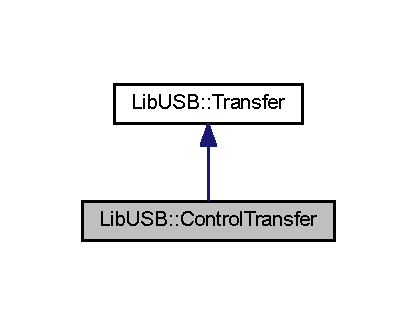
\includegraphics[width=200pt]{class_lib_u_s_b_1_1_control_transfer__inherit__graph}
\end{center}
\end{figure}


Collaboration diagram for Lib\-U\-S\-B\-:\-:Control\-Transfer\-:\nopagebreak
\begin{figure}[H]
\begin{center}
\leavevmode
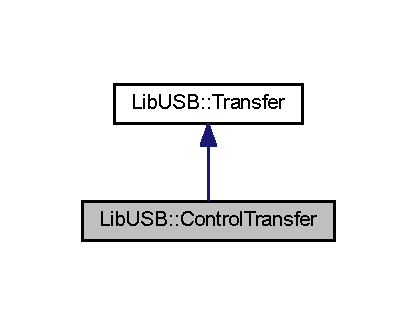
\includegraphics[width=200pt]{class_lib_u_s_b_1_1_control_transfer__coll__graph}
\end{center}
\end{figure}
\subsection*{Public Member Functions}
\begin{DoxyCompactItemize}
\item 
\hypertarget{class_lib_u_s_b_1_1_control_transfer_a8bfafa78c1d745221cf80da5333abd17}{{\bfseries Control\-Transfer} (std\-::shared\-\_\-ptr$<$ Transfer\-Impl $>$ p\-Transfer\-Impl)}\label{class_lib_u_s_b_1_1_control_transfer_a8bfafa78c1d745221cf80da5333abd17}

\item 
\hypertarget{class_lib_u_s_b_1_1_control_transfer_a83d9e5b876cb4654e37168b1bb93f3cd}{virtual void \hyperlink{class_lib_u_s_b_1_1_control_transfer_a83d9e5b876cb4654e37168b1bb93f3cd}{Setup\-Packet} (uint8\-\_\-t Request, uint16\-\_\-t w\-Value, uint16\-\_\-t w\-Index, Data\-Transfer\-Direction\-\_\-t data\-Direction=H\-O\-S\-T\-\_\-\-T\-O\-\_\-\-D\-E\-V\-I\-C\-E, Request\-Type\-\_\-t request\-Type=R\-E\-Q\-\_\-\-V\-E\-N\-D\-O\-R, Request\-Recipient\-\_\-t recipient=R\-E\-C\-\_\-\-E\-N\-D\-P\-O\-I\-N\-T)}\label{class_lib_u_s_b_1_1_control_transfer_a83d9e5b876cb4654e37168b1bb93f3cd}

\begin{DoxyCompactList}\small\item\em U\-S\-B Control transfer setup method. \end{DoxyCompactList}\end{DoxyCompactItemize}
\subsection*{Additional Inherited Members}


\subsection{Detailed Description}
U\-S\-B Control transfer object. 

The documentation for this class was generated from the following file\-:\begin{DoxyCompactItemize}
\item 
headers/Transfer.\-h\end{DoxyCompactItemize}

\hypertarget{class_lib_u_s_b_1_1_device}{\section{Lib\-U\-S\-B\-:\-:Device Class Reference}
\label{class_lib_u_s_b_1_1_device}\index{Lib\-U\-S\-B\-::\-Device@{Lib\-U\-S\-B\-::\-Device}}
}


Libusb device interface.  




{\ttfamily \#include $<$device.\-h$>$}

\subsection*{Public Member Functions}
\begin{DoxyCompactItemize}
\item 
\hypertarget{class_lib_u_s_b_1_1_device_aeaa204a15758e97814f22daef0620bbe}{{\bfseries Device} (std\-::shared\-\_\-ptr$<$ Device\-Impl $>$ p\-Init)}\label{class_lib_u_s_b_1_1_device_aeaa204a15758e97814f22daef0620bbe}

\item 
\hypertarget{class_lib_u_s_b_1_1_device_a243abe3304f5b0df560c1c1d4996fc27}{void {\bfseries Init} ()}\label{class_lib_u_s_b_1_1_device_a243abe3304f5b0df560c1c1d4996fc27}

\item 
\hypertarget{class_lib_u_s_b_1_1_device_aab5f0f101c8ca3e7f3efd22906259a07}{bool \hyperlink{class_lib_u_s_b_1_1_device_aab5f0f101c8ca3e7f3efd22906259a07}{is\-Open} ()}\label{class_lib_u_s_b_1_1_device_aab5f0f101c8ca3e7f3efd22906259a07}

\begin{DoxyCompactList}\small\item\em Returns T\-R\-U\-E if the device is open. \end{DoxyCompactList}\item 
\hypertarget{class_lib_u_s_b_1_1_device_ad3d1cb1906cc40792d91f465d2fa8475}{void \hyperlink{class_lib_u_s_b_1_1_device_ad3d1cb1906cc40792d91f465d2fa8475}{Open} ()}\label{class_lib_u_s_b_1_1_device_ad3d1cb1906cc40792d91f465d2fa8475}

\begin{DoxyCompactList}\small\item\em Opens the device. \end{DoxyCompactList}\item 
\hypertarget{class_lib_u_s_b_1_1_device_a59034f46f295c33e8508fc249d196f3a}{uint16\-\_\-t \hyperlink{class_lib_u_s_b_1_1_device_a59034f46f295c33e8508fc249d196f3a}{U\-S\-B\-Specification} ()}\label{class_lib_u_s_b_1_1_device_a59034f46f295c33e8508fc249d196f3a}

\begin{DoxyCompactList}\small\item\em U\-S\-B specification release number. \end{DoxyCompactList}\item 
\hypertarget{class_lib_u_s_b_1_1_device_a1e20bb4c9f2df68b470dcc6c9922a209}{uint8\-\_\-t \hyperlink{class_lib_u_s_b_1_1_device_a1e20bb4c9f2df68b470dcc6c9922a209}{Device\-Class} ()}\label{class_lib_u_s_b_1_1_device_a1e20bb4c9f2df68b470dcc6c9922a209}

\begin{DoxyCompactList}\small\item\em U\-S\-B-\/\-I\-F class code. \end{DoxyCompactList}\item 
\hypertarget{class_lib_u_s_b_1_1_device_a86766778e062854e0a7d7b264793e9aa}{uint8\-\_\-t \hyperlink{class_lib_u_s_b_1_1_device_a86766778e062854e0a7d7b264793e9aa}{Device\-Subclass} ()}\label{class_lib_u_s_b_1_1_device_a86766778e062854e0a7d7b264793e9aa}

\begin{DoxyCompactList}\small\item\em U\-S\-B-\/\-I\-F subclass code for the device, qualified by the b\-Device\-Class value. \end{DoxyCompactList}\item 
\hypertarget{class_lib_u_s_b_1_1_device_ab3ae560d2ab9bf058d39eb266e752d98}{uint8\-\_\-t \hyperlink{class_lib_u_s_b_1_1_device_ab3ae560d2ab9bf058d39eb266e752d98}{Device\-Protocol} ()}\label{class_lib_u_s_b_1_1_device_ab3ae560d2ab9bf058d39eb266e752d98}

\begin{DoxyCompactList}\small\item\em U\-S\-B-\/\-I\-F protocol code for the device, qualified by the b\-Device\-Class and b\-Device\-Sub\-Class values. \end{DoxyCompactList}\item 
\hypertarget{class_lib_u_s_b_1_1_device_a10d9993286eea8424f0d97bb5a0cbab6}{uint16\-\_\-t \hyperlink{class_lib_u_s_b_1_1_device_a10d9993286eea8424f0d97bb5a0cbab6}{vendor\-I\-D} ()}\label{class_lib_u_s_b_1_1_device_a10d9993286eea8424f0d97bb5a0cbab6}

\begin{DoxyCompactList}\small\item\em U\-S\-B-\/\-I\-F vendor I\-D. \end{DoxyCompactList}\item 
\hypertarget{class_lib_u_s_b_1_1_device_a5f3f9c76a5b6f10e70b71b63dcae575d}{uint16\-\_\-t \hyperlink{class_lib_u_s_b_1_1_device_a5f3f9c76a5b6f10e70b71b63dcae575d}{product\-I\-D} ()}\label{class_lib_u_s_b_1_1_device_a5f3f9c76a5b6f10e70b71b63dcae575d}

\begin{DoxyCompactList}\small\item\em U\-S\-B-\/\-I\-F product I\-D. \end{DoxyCompactList}\item 
\hypertarget{class_lib_u_s_b_1_1_device_a2675fa27b241d017e20a20bd7d7a8af9}{std\-::wstring \hyperlink{class_lib_u_s_b_1_1_device_a2675fa27b241d017e20a20bd7d7a8af9}{Product\-String} ()}\label{class_lib_u_s_b_1_1_device_a2675fa27b241d017e20a20bd7d7a8af9}

\begin{DoxyCompactList}\small\item\em Returns a string describing the product. \end{DoxyCompactList}\item 
\hypertarget{class_lib_u_s_b_1_1_device_a8bdf8188d169b78b6042acdace38029d}{std\-::wstring \hyperlink{class_lib_u_s_b_1_1_device_a8bdf8188d169b78b6042acdace38029d}{Manufacturer\-String} ()}\label{class_lib_u_s_b_1_1_device_a8bdf8188d169b78b6042acdace38029d}

\begin{DoxyCompactList}\small\item\em Returns a string describing the manufacturer. \end{DoxyCompactList}\item 
\hypertarget{class_lib_u_s_b_1_1_device_aab1bf4b42123fe6e83614e49a95c4fcf}{std\-::wstring \hyperlink{class_lib_u_s_b_1_1_device_aab1bf4b42123fe6e83614e49a95c4fcf}{Serial\-String} ()}\label{class_lib_u_s_b_1_1_device_aab1bf4b42123fe6e83614e49a95c4fcf}

\begin{DoxyCompactList}\small\item\em Returns the serial number string of the device. \end{DoxyCompactList}\item 
\hypertarget{class_lib_u_s_b_1_1_device_a38ef4e0bb23c0db89297bbe3f1a7f019}{uint8\-\_\-t \hyperlink{class_lib_u_s_b_1_1_device_a38ef4e0bb23c0db89297bbe3f1a7f019}{Num\-Configurations} ()}\label{class_lib_u_s_b_1_1_device_a38ef4e0bb23c0db89297bbe3f1a7f019}

\begin{DoxyCompactList}\small\item\em Returns the number of possible configurations for this device. \end{DoxyCompactList}\item 
\hypertarget{class_lib_u_s_b_1_1_device_a5ce2cb2d3b4e92fe28f35eb1d5e38b77}{std\-::shared\-\_\-ptr$<$ \hyperlink{class_lib_u_s_b_1_1_configuration}{Configuration} $>$ \hyperlink{class_lib_u_s_b_1_1_device_a5ce2cb2d3b4e92fe28f35eb1d5e38b77}{get\-Configuration} (uint8\-\_\-t Config\-Value)}\label{class_lib_u_s_b_1_1_device_a5ce2cb2d3b4e92fe28f35eb1d5e38b77}

\begin{DoxyCompactList}\small\item\em Returns the requested configuration. \end{DoxyCompactList}\item 
\hypertarget{class_lib_u_s_b_1_1_device_a586bcbb3872d1f079fae9f1b6ae96ef4}{std\-::shared\-\_\-ptr$<$ \hyperlink{class_lib_u_s_b_1_1_configuration}{Configuration} $>$ \hyperlink{class_lib_u_s_b_1_1_device_a586bcbb3872d1f079fae9f1b6ae96ef4}{get\-Active\-Configuration} ()}\label{class_lib_u_s_b_1_1_device_a586bcbb3872d1f079fae9f1b6ae96ef4}

\begin{DoxyCompactList}\small\item\em Returns the active\-Configuration. \end{DoxyCompactList}\item 
\hypertarget{class_lib_u_s_b_1_1_device_a0d24eae437e17a93ccdfa2a249650fc5}{std\-::shared\-\_\-ptr$<$ \hyperlink{class_lib_u_s_b_1_1_endpoint}{Endpoint} $>$ \hyperlink{class_lib_u_s_b_1_1_device_a0d24eae437e17a93ccdfa2a249650fc5}{get\-Control\-Endpoint} ()}\label{class_lib_u_s_b_1_1_device_a0d24eae437e17a93ccdfa2a249650fc5}

\begin{DoxyCompactList}\small\item\em Returns the control endpoint (\hyperlink{class_lib_u_s_b_1_1_endpoint}{Endpoint} 0) \end{DoxyCompactList}\end{DoxyCompactItemize}
\subsection*{Protected Member Functions}
\begin{DoxyCompactItemize}
\item 
virtual void \hyperlink{class_lib_u_s_b_1_1_device_a2b7f495eb8c2693602f212c2c2773f15}{Transfer\-Event\-Notification} (std\-::shared\-\_\-ptr$<$ \hyperlink{class_lib_u_s_b_1_1_transfer}{Transfer} $>$ p\-Completed\-Transfer)
\end{DoxyCompactItemize}
\subsection*{Friends}
\begin{DoxyCompactItemize}
\item 
\hypertarget{class_lib_u_s_b_1_1_device_aed9f2bd8ff81bd3986d935f9aa242d1b}{class \hyperlink{class_lib_u_s_b_1_1_device_aed9f2bd8ff81bd3986d935f9aa242d1b}{Transfer\-Impl}}\label{class_lib_u_s_b_1_1_device_aed9f2bd8ff81bd3986d935f9aa242d1b}

\begin{DoxyCompactList}\small\item\em Transfers need access to the transfer event notification method of their target device. \end{DoxyCompactList}\end{DoxyCompactItemize}


\subsection{Detailed Description}
Libusb device interface. 

\subsection{Member Function Documentation}
\hypertarget{class_lib_u_s_b_1_1_device_a2b7f495eb8c2693602f212c2c2773f15}{\index{Lib\-U\-S\-B\-::\-Device@{Lib\-U\-S\-B\-::\-Device}!Transfer\-Event\-Notification@{Transfer\-Event\-Notification}}
\index{Transfer\-Event\-Notification@{Transfer\-Event\-Notification}!LibUSB::Device@{Lib\-U\-S\-B\-::\-Device}}
\subsubsection[{Transfer\-Event\-Notification}]{\setlength{\rightskip}{0pt plus 5cm}virtual void Lib\-U\-S\-B\-::\-Device\-::\-Transfer\-Event\-Notification (
\begin{DoxyParamCaption}
\item[{std\-::shared\-\_\-ptr$<$ {\bf Transfer} $>$}]{p\-Completed\-Transfer}
\end{DoxyParamCaption}
)\hspace{0.3cm}{\ttfamily [protected]}, {\ttfamily [virtual]}}}\label{class_lib_u_s_b_1_1_device_a2b7f495eb8c2693602f212c2c2773f15}
Notification of a completed transfer \begin{DoxyWarning}{Warning}
This function can be called from other threads when using asynchronous transfers! 
\end{DoxyWarning}


The documentation for this class was generated from the following file\-:\begin{DoxyCompactItemize}
\item 
headers/device.\-h\end{DoxyCompactItemize}

\hypertarget{class_lib_u_s_b_1_1_endpoint}{\section{Lib\-U\-S\-B\-:\-:Endpoint Class Reference}
\label{class_lib_u_s_b_1_1_endpoint}\index{Lib\-U\-S\-B\-::\-Endpoint@{Lib\-U\-S\-B\-::\-Endpoint}}
}


U\-S\-B endpoint class.  




{\ttfamily \#include $<$Endpoint.\-h$>$}

\subsection*{Public Member Functions}
\begin{DoxyCompactItemize}
\item 
\hypertarget{class_lib_u_s_b_1_1_endpoint_a6916ca81cbe5dc84487041ef4269afb6}{{\bfseries Endpoint} (std\-::shared\-\_\-ptr$<$ Endpoint\-Impl $>$ p\-Impl)}\label{class_lib_u_s_b_1_1_endpoint_a6916ca81cbe5dc84487041ef4269afb6}

\item 
\hypertarget{class_lib_u_s_b_1_1_endpoint_a87324673d0521e6a87181d734843797a}{uint8\-\_\-t \hyperlink{class_lib_u_s_b_1_1_endpoint_a87324673d0521e6a87181d734843797a}{Address} () const }\label{class_lib_u_s_b_1_1_endpoint_a87324673d0521e6a87181d734843797a}

\begin{DoxyCompactList}\small\item\em Raw \hyperlink{class_lib_u_s_b_1_1_endpoint}{Endpoint} Address. \end{DoxyCompactList}\item 
\hypertarget{class_lib_u_s_b_1_1_endpoint_a16f5d238ac0f007dbf22b51b2521278c}{int \hyperlink{class_lib_u_s_b_1_1_endpoint_a16f5d238ac0f007dbf22b51b2521278c}{Number} () const }\label{class_lib_u_s_b_1_1_endpoint_a16f5d238ac0f007dbf22b51b2521278c}

\begin{DoxyCompactList}\small\item\em \hyperlink{class_lib_u_s_b_1_1_endpoint}{Endpoint} Number. \end{DoxyCompactList}\item 
\hypertarget{class_lib_u_s_b_1_1_endpoint_a27e288784eaf72a217435e8f5d920d43}{Direction\-\_\-t \hyperlink{class_lib_u_s_b_1_1_endpoint_a27e288784eaf72a217435e8f5d920d43}{Direction} () const }\label{class_lib_u_s_b_1_1_endpoint_a27e288784eaf72a217435e8f5d920d43}

\begin{DoxyCompactList}\small\item\em Returns the direction of this endpoint. \end{DoxyCompactList}\item 
\hypertarget{class_lib_u_s_b_1_1_endpoint_aa5b591898f33c0e2c684c22dadf50974}{Transfer\-\_\-t \hyperlink{class_lib_u_s_b_1_1_endpoint_aa5b591898f33c0e2c684c22dadf50974}{Transfer\-Type} () const }\label{class_lib_u_s_b_1_1_endpoint_aa5b591898f33c0e2c684c22dadf50974}

\begin{DoxyCompactList}\small\item\em Returns the transfer type of this endpoint. \end{DoxyCompactList}\item 
\hypertarget{class_lib_u_s_b_1_1_endpoint_a7cfbe2c62da0e8c84587ed05dc82a1e6}{Synchronization\-\_\-t \hyperlink{class_lib_u_s_b_1_1_endpoint_a7cfbe2c62da0e8c84587ed05dc82a1e6}{Synchronization\-Type} () const }\label{class_lib_u_s_b_1_1_endpoint_a7cfbe2c62da0e8c84587ed05dc82a1e6}

\begin{DoxyCompactList}\small\item\em Returns the synchronization type (I\-S\-O\-C\-H\-R\-O\-N\-O\-U\-S M\-O\-D\-E O\-N\-L\-Y!) \end{DoxyCompactList}\item 
\hypertarget{class_lib_u_s_b_1_1_endpoint_ad25de43b4d384489061382311505deed}{Usage\-\_\-t \hyperlink{class_lib_u_s_b_1_1_endpoint_ad25de43b4d384489061382311505deed}{Usage\-Type} () const }\label{class_lib_u_s_b_1_1_endpoint_ad25de43b4d384489061382311505deed}

\begin{DoxyCompactList}\small\item\em Returns the usage type (I\-S\-O\-C\-H\-R\-O\-N\-O\-U\-S M\-O\-D\-E O\-N\-L\-Y!) \end{DoxyCompactList}\item 
\hypertarget{class_lib_u_s_b_1_1_endpoint_a82abc743029a6ae25950509b0a389c7b}{int \hyperlink{class_lib_u_s_b_1_1_endpoint_a82abc743029a6ae25950509b0a389c7b}{Max\-Packet\-Size} () const }\label{class_lib_u_s_b_1_1_endpoint_a82abc743029a6ae25950509b0a389c7b}

\begin{DoxyCompactList}\small\item\em Returns the maximum packet size for this endpoint. \end{DoxyCompactList}\item 
\hypertarget{class_lib_u_s_b_1_1_endpoint_a5082b5c139a3585d8b7277a273c1effc}{int \hyperlink{class_lib_u_s_b_1_1_endpoint_a5082b5c139a3585d8b7277a273c1effc}{Polling\-Interval} () const }\label{class_lib_u_s_b_1_1_endpoint_a5082b5c139a3585d8b7277a273c1effc}

\begin{DoxyCompactList}\small\item\em Returns the polling interval (in frames, 1f = 1m\-S @ low/full speed, 125u\-S at high), ignore for bulk/control, 1 for iso, 1-\/255 for interrupt. \end{DoxyCompactList}\item 
\hypertarget{class_lib_u_s_b_1_1_endpoint_a70135be407240a2577da526217f4d742}{std\-::shared\-\_\-ptr$<$ \hyperlink{class_lib_u_s_b_1_1_transfer}{Transfer} $>$ \hyperlink{class_lib_u_s_b_1_1_endpoint_a70135be407240a2577da526217f4d742}{Create\-Transfer} ()}\label{class_lib_u_s_b_1_1_endpoint_a70135be407240a2577da526217f4d742}

\begin{DoxyCompactList}\small\item\em Creates a new data transfer object. \end{DoxyCompactList}\end{DoxyCompactItemize}


\subsection{Detailed Description}
U\-S\-B endpoint class. 

The documentation for this class was generated from the following file\-:\begin{DoxyCompactItemize}
\item 
headers/Endpoint.\-h\end{DoxyCompactItemize}

\hypertarget{class_lib_u_s_b_1_1_interface}{\section{Lib\-U\-S\-B\-:\-:Interface Class Reference}
\label{class_lib_u_s_b_1_1_interface}\index{Lib\-U\-S\-B\-::\-Interface@{Lib\-U\-S\-B\-::\-Interface}}
}


U\-S\-B \hyperlink{class_lib_u_s_b_1_1_interface}{Interface} class.  




{\ttfamily \#include $<$Interface.\-h$>$}

\subsection*{Public Member Functions}
\begin{DoxyCompactItemize}
\item 
\hypertarget{class_lib_u_s_b_1_1_interface_a7f338d55d22c5f8916c7f60fdd53712c}{{\bfseries Interface} (std\-::shared\-\_\-ptr$<$ Interface\-Impl $>$ p\-Impl)}\label{class_lib_u_s_b_1_1_interface_a7f338d55d22c5f8916c7f60fdd53712c}

\item 
\hypertarget{class_lib_u_s_b_1_1_interface_a481db81fa12cf6324162be7bdf8a53bb}{int \hyperlink{class_lib_u_s_b_1_1_interface_a481db81fa12cf6324162be7bdf8a53bb}{Number} () const }\label{class_lib_u_s_b_1_1_interface_a481db81fa12cf6324162be7bdf8a53bb}

\begin{DoxyCompactList}\small\item\em Returns the interface number. \end{DoxyCompactList}\item 
\hypertarget{class_lib_u_s_b_1_1_interface_a52b602b375dc3e53b2c6c3bafb7be3d7}{int \hyperlink{class_lib_u_s_b_1_1_interface_a52b602b375dc3e53b2c6c3bafb7be3d7}{Alternate\-Setting} () const }\label{class_lib_u_s_b_1_1_interface_a52b602b375dc3e53b2c6c3bafb7be3d7}

\begin{DoxyCompactList}\small\item\em Returns the alternate setting for this interface. \end{DoxyCompactList}\item 
\hypertarget{class_lib_u_s_b_1_1_interface_a5e87fddb4aa5f1e859058ee9bd2a02f7}{int \hyperlink{class_lib_u_s_b_1_1_interface_a5e87fddb4aa5f1e859058ee9bd2a02f7}{Class} () const }\label{class_lib_u_s_b_1_1_interface_a5e87fddb4aa5f1e859058ee9bd2a02f7}

\begin{DoxyCompactList}\small\item\em Returns the interface class. \end{DoxyCompactList}\item 
\hypertarget{class_lib_u_s_b_1_1_interface_ab5fcfdab1f342dc7096c3f8b0d7ebd9b}{int \hyperlink{class_lib_u_s_b_1_1_interface_ab5fcfdab1f342dc7096c3f8b0d7ebd9b}{Sub\-Class} () const }\label{class_lib_u_s_b_1_1_interface_ab5fcfdab1f342dc7096c3f8b0d7ebd9b}

\begin{DoxyCompactList}\small\item\em Returns the interface Subclass. \end{DoxyCompactList}\item 
\hypertarget{class_lib_u_s_b_1_1_interface_a67ded20edf389d021702a4face74d70d}{int \hyperlink{class_lib_u_s_b_1_1_interface_a67ded20edf389d021702a4face74d70d}{Protocol} () const }\label{class_lib_u_s_b_1_1_interface_a67ded20edf389d021702a4face74d70d}

\begin{DoxyCompactList}\small\item\em Returns the interface Protocol. \end{DoxyCompactList}\item 
\hypertarget{class_lib_u_s_b_1_1_interface_a7e5da83b8c77cd2ec43da8e2917d2383}{std\-::wstring \hyperlink{class_lib_u_s_b_1_1_interface_a7e5da83b8c77cd2ec43da8e2917d2383}{Descriptor\-String} () const }\label{class_lib_u_s_b_1_1_interface_a7e5da83b8c77cd2ec43da8e2917d2383}

\begin{DoxyCompactList}\small\item\em Returns a string descriptor for this interface. \end{DoxyCompactList}\item 
\hypertarget{class_lib_u_s_b_1_1_interface_a6bb6c4d5cea3a7d6e6e927afd36a30c1}{int \hyperlink{class_lib_u_s_b_1_1_interface_a6bb6c4d5cea3a7d6e6e927afd36a30c1}{Num\-Alternate\-Settings} () const }\label{class_lib_u_s_b_1_1_interface_a6bb6c4d5cea3a7d6e6e927afd36a30c1}

\begin{DoxyCompactList}\small\item\em Returns the number of available alternate settings for this interface. \end{DoxyCompactList}\item 
\hypertarget{class_lib_u_s_b_1_1_interface_a38e98dcd6c3d9878f0070ddb207de1db}{void \hyperlink{class_lib_u_s_b_1_1_interface_a38e98dcd6c3d9878f0070ddb207de1db}{Claim} ()}\label{class_lib_u_s_b_1_1_interface_a38e98dcd6c3d9878f0070ddb207de1db}

\begin{DoxyCompactList}\small\item\em Claims this interface for use. \end{DoxyCompactList}\item 
\hypertarget{class_lib_u_s_b_1_1_interface_a3647afca72cc33775f2a55de354e1a99}{bool \hyperlink{class_lib_u_s_b_1_1_interface_a3647afca72cc33775f2a55de354e1a99}{is\-Claimed} () const }\label{class_lib_u_s_b_1_1_interface_a3647afca72cc33775f2a55de354e1a99}

\begin{DoxyCompactList}\small\item\em Returns T\-R\-U\-E if the interface is claimed. \end{DoxyCompactList}\item 
\hypertarget{class_lib_u_s_b_1_1_interface_a3ab6a262cc1475ea119729838aca6de6}{void \hyperlink{class_lib_u_s_b_1_1_interface_a3ab6a262cc1475ea119729838aca6de6}{Release} ()}\label{class_lib_u_s_b_1_1_interface_a3ab6a262cc1475ea119729838aca6de6}

\begin{DoxyCompactList}\small\item\em Releases this interface. \end{DoxyCompactList}\item 
\hypertarget{class_lib_u_s_b_1_1_interface_a804fe82696522bd7dee8d7629d95c24a}{void \hyperlink{class_lib_u_s_b_1_1_interface_a804fe82696522bd7dee8d7629d95c24a}{Set\-Alternate} (uint8\-\_\-t \hyperlink{class_lib_u_s_b_1_1_interface_a52b602b375dc3e53b2c6c3bafb7be3d7}{Alternate\-Setting}=0)}\label{class_lib_u_s_b_1_1_interface_a804fe82696522bd7dee8d7629d95c24a}

\begin{DoxyCompactList}\small\item\em Sets the requested alternate setting. \end{DoxyCompactList}\item 
\hypertarget{class_lib_u_s_b_1_1_interface_a80e1ca389b48139974d43f3c194f1c2a}{int \hyperlink{class_lib_u_s_b_1_1_interface_a80e1ca389b48139974d43f3c194f1c2a}{Num\-Endpoints} () const }\label{class_lib_u_s_b_1_1_interface_a80e1ca389b48139974d43f3c194f1c2a}

\begin{DoxyCompactList}\small\item\em Returns the number of endpoints this interface has. \end{DoxyCompactList}\item 
\hypertarget{class_lib_u_s_b_1_1_interface_a79d86a85d4ef11cada54bdc192a9e3b5}{std\-::shared\-\_\-ptr$<$ \hyperlink{class_lib_u_s_b_1_1_endpoint}{Endpoint} $>$ \hyperlink{class_lib_u_s_b_1_1_interface_a79d86a85d4ef11cada54bdc192a9e3b5}{get\-Endpoint} (int index)}\label{class_lib_u_s_b_1_1_interface_a79d86a85d4ef11cada54bdc192a9e3b5}

\begin{DoxyCompactList}\small\item\em Returns the specified endpoint. \end{DoxyCompactList}\end{DoxyCompactItemize}


\subsection{Detailed Description}
U\-S\-B \hyperlink{class_lib_u_s_b_1_1_interface}{Interface} class. 

The documentation for this class was generated from the following file\-:\begin{DoxyCompactItemize}
\item 
headers/Interface.\-h\end{DoxyCompactItemize}

\hypertarget{class_lib_u_s_b_1_1_interrupt_transfer}{\section{Lib\-U\-S\-B\-:\-:Interrupt\-Transfer Class Reference}
\label{class_lib_u_s_b_1_1_interrupt_transfer}\index{Lib\-U\-S\-B\-::\-Interrupt\-Transfer@{Lib\-U\-S\-B\-::\-Interrupt\-Transfer}}
}


U\-S\-B Interrupt \hyperlink{class_lib_u_s_b_1_1_transfer}{Transfer} object.  




{\ttfamily \#include $<$Transfer.\-h$>$}



Inheritance diagram for Lib\-U\-S\-B\-:\-:Interrupt\-Transfer\-:\nopagebreak
\begin{figure}[H]
\begin{center}
\leavevmode
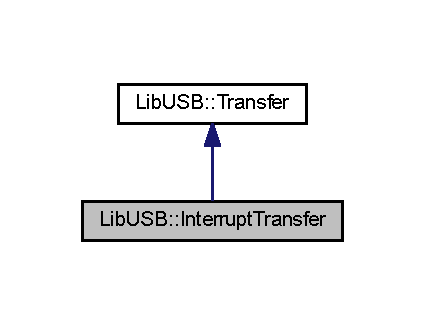
\includegraphics[width=204pt]{class_lib_u_s_b_1_1_interrupt_transfer__inherit__graph}
\end{center}
\end{figure}


Collaboration diagram for Lib\-U\-S\-B\-:\-:Interrupt\-Transfer\-:\nopagebreak
\begin{figure}[H]
\begin{center}
\leavevmode
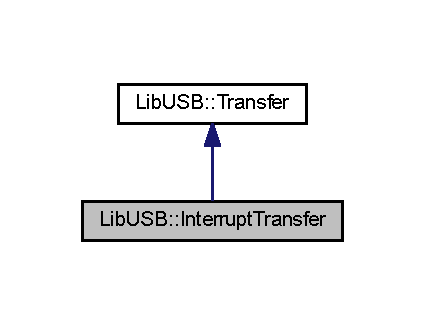
\includegraphics[width=204pt]{class_lib_u_s_b_1_1_interrupt_transfer__coll__graph}
\end{center}
\end{figure}
\subsection*{Public Member Functions}
\begin{DoxyCompactItemize}
\item 
\hypertarget{class_lib_u_s_b_1_1_interrupt_transfer_a79401af995e4992996ac716a2fa223ba}{{\bfseries Interrupt\-Transfer} (std\-::shared\-\_\-ptr$<$ Transfer\-Impl $>$ p\-Transfer\-Impl)}\label{class_lib_u_s_b_1_1_interrupt_transfer_a79401af995e4992996ac716a2fa223ba}

\end{DoxyCompactItemize}
\subsection*{Additional Inherited Members}


\subsection{Detailed Description}
U\-S\-B Interrupt \hyperlink{class_lib_u_s_b_1_1_transfer}{Transfer} object. 

The documentation for this class was generated from the following file\-:\begin{DoxyCompactItemize}
\item 
headers/Transfer.\-h\end{DoxyCompactItemize}

\hypertarget{class_lib_u_s_b_1_1_isochronous_transfer}{\section{Lib\-U\-S\-B\-:\-:Isochronous\-Transfer Class Reference}
\label{class_lib_u_s_b_1_1_isochronous_transfer}\index{Lib\-U\-S\-B\-::\-Isochronous\-Transfer@{Lib\-U\-S\-B\-::\-Isochronous\-Transfer}}
}


U\-S\-B Isochronous \hyperlink{class_lib_u_s_b_1_1_transfer}{Transfer} object.  




{\ttfamily \#include $<$Transfer.\-h$>$}



Inheritance diagram for Lib\-U\-S\-B\-:\-:Isochronous\-Transfer\-:\nopagebreak
\begin{figure}[H]
\begin{center}
\leavevmode
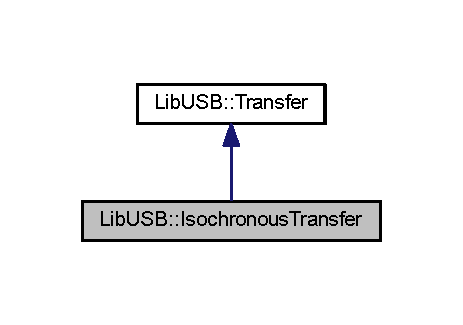
\includegraphics[width=222pt]{class_lib_u_s_b_1_1_isochronous_transfer__inherit__graph}
\end{center}
\end{figure}


Collaboration diagram for Lib\-U\-S\-B\-:\-:Isochronous\-Transfer\-:\nopagebreak
\begin{figure}[H]
\begin{center}
\leavevmode
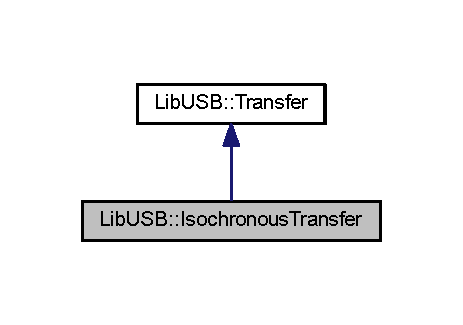
\includegraphics[width=222pt]{class_lib_u_s_b_1_1_isochronous_transfer__coll__graph}
\end{center}
\end{figure}
\subsection*{Public Member Functions}
\begin{DoxyCompactItemize}
\item 
\hypertarget{class_lib_u_s_b_1_1_isochronous_transfer_a1b5761f6dd930b29eba85b8088d29e82}{{\bfseries Isochronous\-Transfer} (std\-::shared\-\_\-ptr$<$ Transfer\-Impl $>$ p\-Transfer\-Impl)}\label{class_lib_u_s_b_1_1_isochronous_transfer_a1b5761f6dd930b29eba85b8088d29e82}

\item 
\hypertarget{class_lib_u_s_b_1_1_isochronous_transfer_a97399b533b68a340b31b690571ce57fa}{void \hyperlink{class_lib_u_s_b_1_1_isochronous_transfer_a97399b533b68a340b31b690571ce57fa}{set\-Num\-Packets} (int Packets)}\label{class_lib_u_s_b_1_1_isochronous_transfer_a97399b533b68a340b31b690571ce57fa}

\begin{DoxyCompactList}\small\item\em Sets the number of packets. \end{DoxyCompactList}\end{DoxyCompactItemize}
\subsection*{Additional Inherited Members}


\subsection{Detailed Description}
U\-S\-B Isochronous \hyperlink{class_lib_u_s_b_1_1_transfer}{Transfer} object. 

The documentation for this class was generated from the following file\-:\begin{DoxyCompactItemize}
\item 
headers/Transfer.\-h\end{DoxyCompactItemize}

\hypertarget{class_lib_u_s_b_1_1_lib_u_s_b}{\section{Lib\-U\-S\-B\-:\-:Lib\-U\-S\-B Class Reference}
\label{class_lib_u_s_b_1_1_lib_u_s_b}\index{Lib\-U\-S\-B\-::\-Lib\-U\-S\-B@{Lib\-U\-S\-B\-::\-Lib\-U\-S\-B}}
}


Contains static methods for enumerating devices.  




{\ttfamily \#include $<$libusbpp.\-h$>$}

\subsection*{Public Types}
\begin{DoxyCompactItemize}
\item 
typedef std\-::shared\-\_\-ptr$<$ \hyperlink{class_lib_u_s_b_1_1_device}{Device} $>$($\ast$ \hyperlink{class_lib_u_s_b_1_1_lib_u_s_b_a532d474d390477dffd2109e8540be558}{Device\-Factory\-\_\-t} )(std\-::shared\-\_\-ptr$<$ Device\-Impl $>$)
\end{DoxyCompactItemize}
\subsection*{Static Public Member Functions}
\begin{DoxyCompactItemize}
\item 
static std\-::list\\*
$<$ std\-::shared\-\_\-ptr$<$ \hyperlink{class_lib_u_s_b_1_1_device}{Device} $>$ $>$ \hyperlink{class_lib_u_s_b_1_1_lib_u_s_b_a1e96edfe8903783e33d572ff43ee8238}{Find\-Device} (uint16\-\_\-t vendor\-I\-D, uint16\-\_\-t product\-I\-D, \hyperlink{class_lib_u_s_b_1_1_lib_u_s_b_a532d474d390477dffd2109e8540be558}{Device\-Factory\-\_\-t} factory=nullptr)
\begin{DoxyCompactList}\small\item\em Returns a list of devices (that can be opened) that match the given vendor/product id. \end{DoxyCompactList}\item 
static std\-::list\\*
$<$ std\-::shared\-\_\-ptr$<$ \hyperlink{class_lib_u_s_b_1_1_device}{Device} $>$ $>$ \hyperlink{class_lib_u_s_b_1_1_lib_u_s_b_aaf1f6d3a7df3a9fefd8b12ba25a7c3be}{Find\-Device} (uint16\-\_\-t vendor\-I\-D, uint16\-\_\-t product\-I\-D, std\-::wstring serial\-Str, \hyperlink{class_lib_u_s_b_1_1_lib_u_s_b_a532d474d390477dffd2109e8540be558}{Device\-Factory\-\_\-t} factory=nullptr)
\begin{DoxyCompactList}\small\item\em Returns a list of devices (that can be opened) that match the given vendor/product id. \end{DoxyCompactList}\item 
\hypertarget{class_lib_u_s_b_1_1_lib_u_s_b_acce20c7a3bd52fffe9df3ce23021858d}{static std\-::list\\*
$<$ std\-::shared\-\_\-ptr$<$ \hyperlink{class_lib_u_s_b_1_1_device}{Device} $>$ $>$ \hyperlink{class_lib_u_s_b_1_1_lib_u_s_b_acce20c7a3bd52fffe9df3ce23021858d}{Find\-All\-Devices} (\hyperlink{class_lib_u_s_b_1_1_lib_u_s_b_a532d474d390477dffd2109e8540be558}{Device\-Factory\-\_\-t} factory=nullptr)}\label{class_lib_u_s_b_1_1_lib_u_s_b_acce20c7a3bd52fffe9df3ce23021858d}

\begin{DoxyCompactList}\small\item\em Returns all devices attached to the system. \end{DoxyCompactList}\end{DoxyCompactItemize}
\subsection*{Friends}
\begin{DoxyCompactItemize}
\item 
\hypertarget{class_lib_u_s_b_1_1_lib_u_s_b_aed9f2bd8ff81bd3986d935f9aa242d1b}{class {\bfseries Transfer\-Impl}}\label{class_lib_u_s_b_1_1_lib_u_s_b_aed9f2bd8ff81bd3986d935f9aa242d1b}

\end{DoxyCompactItemize}


\subsection{Detailed Description}
Contains static methods for enumerating devices. 

\subsection{Member Typedef Documentation}
\hypertarget{class_lib_u_s_b_1_1_lib_u_s_b_a532d474d390477dffd2109e8540be558}{\index{Lib\-U\-S\-B\-::\-Lib\-U\-S\-B@{Lib\-U\-S\-B\-::\-Lib\-U\-S\-B}!Device\-Factory\-\_\-t@{Device\-Factory\-\_\-t}}
\index{Device\-Factory\-\_\-t@{Device\-Factory\-\_\-t}!LibUSB::LibUSB@{Lib\-U\-S\-B\-::\-Lib\-U\-S\-B}}
\subsubsection[{Device\-Factory\-\_\-t}]{\setlength{\rightskip}{0pt plus 5cm}typedef std\-::shared\-\_\-ptr$<${\bf Device}$>$($\ast$ Lib\-U\-S\-B\-::\-Lib\-U\-S\-B\-::\-Device\-Factory\-\_\-t)(std\-::shared\-\_\-ptr$<$ Device\-Impl $>$)}}\label{class_lib_u_s_b_1_1_lib_u_s_b_a532d474d390477dffd2109e8540be558}
Function pointer to a \hyperlink{class_lib_u_s_b_1_1_lib_u_s_b}{Lib\-U\-S\-B} device object factory. \begin{DoxyRefDesc}{Todo}
\item[\hyperlink{todo__todo000001}{Todo}]Replace with std\-::function? \end{DoxyRefDesc}


\subsection{Member Function Documentation}
\hypertarget{class_lib_u_s_b_1_1_lib_u_s_b_a1e96edfe8903783e33d572ff43ee8238}{\index{Lib\-U\-S\-B\-::\-Lib\-U\-S\-B@{Lib\-U\-S\-B\-::\-Lib\-U\-S\-B}!Find\-Device@{Find\-Device}}
\index{Find\-Device@{Find\-Device}!LibUSB::LibUSB@{Lib\-U\-S\-B\-::\-Lib\-U\-S\-B}}
\subsubsection[{Find\-Device}]{\setlength{\rightskip}{0pt plus 5cm}static std\-::list$<$std\-::shared\-\_\-ptr$<${\bf Device}$>$ $>$ Lib\-U\-S\-B\-::\-Lib\-U\-S\-B\-::\-Find\-Device (
\begin{DoxyParamCaption}
\item[{uint16\-\_\-t}]{vendor\-I\-D, }
\item[{uint16\-\_\-t}]{product\-I\-D, }
\item[{{\bf Device\-Factory\-\_\-t}}]{factory = {\ttfamily nullptr}}
\end{DoxyParamCaption}
)\hspace{0.3cm}{\ttfamily [static]}}}\label{class_lib_u_s_b_1_1_lib_u_s_b_a1e96edfe8903783e33d572ff43ee8238}


Returns a list of devices (that can be opened) that match the given vendor/product id. 


\begin{DoxyParams}{Parameters}
{\em vendor\-I\-D} & (uint16\-\_\-t)\-: U\-S\-B-\/\-I\-F vendor id of the desired device. \\
\hline
{\em device\-I\-D} & (uint16\-\_\-t)\-: U\-S\-B-\/\-I\-F product id of the desired device. \\
\hline
\end{DoxyParams}
\begin{DoxyReturn}{Returns}
(std\-::list$<$std\-::shared\-\_\-ptr$<$\-D$>$$>$)\-: List of shared pointers to \hyperlink{class_lib_u_s_b_1_1_device}{Lib\-U\-S\-B\-::\-Device} class objects. 
\end{DoxyReturn}
\begin{DoxySeeAlso}{See Also}

\end{DoxySeeAlso}
\begin{DoxyNote}{Note}

\end{DoxyNote}
\begin{DoxyWarning}{Warning}
Multiple devices can be returned via this method, if attached. 
\end{DoxyWarning}
\hypertarget{class_lib_u_s_b_1_1_lib_u_s_b_aaf1f6d3a7df3a9fefd8b12ba25a7c3be}{\index{Lib\-U\-S\-B\-::\-Lib\-U\-S\-B@{Lib\-U\-S\-B\-::\-Lib\-U\-S\-B}!Find\-Device@{Find\-Device}}
\index{Find\-Device@{Find\-Device}!LibUSB::LibUSB@{Lib\-U\-S\-B\-::\-Lib\-U\-S\-B}}
\subsubsection[{Find\-Device}]{\setlength{\rightskip}{0pt plus 5cm}static std\-::list$<$std\-::shared\-\_\-ptr$<${\bf Device}$>$ $>$ Lib\-U\-S\-B\-::\-Lib\-U\-S\-B\-::\-Find\-Device (
\begin{DoxyParamCaption}
\item[{uint16\-\_\-t}]{vendor\-I\-D, }
\item[{uint16\-\_\-t}]{product\-I\-D, }
\item[{std\-::wstring}]{serial\-Str, }
\item[{{\bf Device\-Factory\-\_\-t}}]{factory = {\ttfamily nullptr}}
\end{DoxyParamCaption}
)\hspace{0.3cm}{\ttfamily [static]}}}\label{class_lib_u_s_b_1_1_lib_u_s_b_aaf1f6d3a7df3a9fefd8b12ba25a7c3be}


Returns a list of devices (that can be opened) that match the given vendor/product id. 


\begin{DoxyParams}{Parameters}
{\em vendor\-I\-D} & (uint16\-\_\-t)\-: U\-S\-B-\/\-I\-F vendor id of the desired device. \\
\hline
{\em device\-I\-D} & (uint16\-\_\-t)\-: U\-S\-B-\/\-I\-F product id of the desired device. \\
\hline
{\em serial\-Str} & (std\-::wstring)\-: \hyperlink{class_lib_u_s_b_1_1_device}{Device} unique serial number \\
\hline
\end{DoxyParams}
\begin{DoxyReturn}{Returns}
(std\-::list$<$std\-::shared\-\_\-ptr$<$\-D$>$$>$)\-: List of shared pointers to \hyperlink{class_lib_u_s_b_1_1_device}{Lib\-U\-S\-B\-::\-Device} class objects. 
\end{DoxyReturn}
\begin{DoxySeeAlso}{See Also}

\end{DoxySeeAlso}
\begin{DoxyNote}{Note}

\end{DoxyNote}
\begin{DoxyWarning}{Warning}
Multiple devices can be returned via this method, if attached. 
\end{DoxyWarning}


The documentation for this class was generated from the following file\-:\begin{DoxyCompactItemize}
\item 
headers/libusbpp.\-h\end{DoxyCompactItemize}

\hypertarget{class_lib_u_s_b_1_1_lib_u_s_b_exception}{\section{Lib\-U\-S\-B\-:\-:Lib\-U\-S\-B\-Exception Class Reference}
\label{class_lib_u_s_b_1_1_lib_u_s_b_exception}\index{Lib\-U\-S\-B\-::\-Lib\-U\-S\-B\-Exception@{Lib\-U\-S\-B\-::\-Lib\-U\-S\-B\-Exception}}
}
\subsection*{Public Member Functions}
\begin{DoxyCompactItemize}
\item 
\hypertarget{class_lib_u_s_b_1_1_lib_u_s_b_exception_ab6e9f0079def8ba7d351922337a91e32}{{\bfseries Lib\-U\-S\-B\-Exception} (std\-::string text, int error\-Code)}\label{class_lib_u_s_b_1_1_lib_u_s_b_exception_ab6e9f0079def8ba7d351922337a91e32}

\item 
\hypertarget{class_lib_u_s_b_1_1_lib_u_s_b_exception_ae269c1b05e34aa58bea037999d327848}{std\-::string {\bfseries translate\-Error} (int Error\-Code)}\label{class_lib_u_s_b_1_1_lib_u_s_b_exception_ae269c1b05e34aa58bea037999d327848}

\item 
\hypertarget{class_lib_u_s_b_1_1_lib_u_s_b_exception_a2a64f523c22d02a51131b43686c8c75f}{int \hyperlink{class_lib_u_s_b_1_1_lib_u_s_b_exception_a2a64f523c22d02a51131b43686c8c75f}{get\-Libusb\-Error\-Code} () const }\label{class_lib_u_s_b_1_1_lib_u_s_b_exception_a2a64f523c22d02a51131b43686c8c75f}

\begin{DoxyCompactList}\small\item\em Returns the raw libusb error code. \end{DoxyCompactList}\item 
\hypertarget{class_lib_u_s_b_1_1_lib_u_s_b_exception_aedc3594fd518b3ba24e45f97b429a428}{virtual const char $\ast$ {\bfseries what} ()}\label{class_lib_u_s_b_1_1_lib_u_s_b_exception_aedc3594fd518b3ba24e45f97b429a428}

\end{DoxyCompactItemize}
\subsection*{Protected Attributes}
\begin{DoxyCompactItemize}
\item 
\hypertarget{class_lib_u_s_b_1_1_lib_u_s_b_exception_acb9f57634841a024e7222c66433042ff}{int {\bfseries m\-\_\-\-Error\-Code}}\label{class_lib_u_s_b_1_1_lib_u_s_b_exception_acb9f57634841a024e7222c66433042ff}

\end{DoxyCompactItemize}


The documentation for this class was generated from the following file\-:\begin{DoxyCompactItemize}
\item 
headers/usbexception.\-h\end{DoxyCompactItemize}

\hypertarget{class_lib_u_s_b_1_1_transfer}{\section{Lib\-U\-S\-B\-:\-:Transfer Class Reference}
\label{class_lib_u_s_b_1_1_transfer}\index{Lib\-U\-S\-B\-::\-Transfer@{Lib\-U\-S\-B\-::\-Transfer}}
}


U\-S\-B Data transfer object.  




{\ttfamily \#include $<$Transfer.\-h$>$}



Inheritance diagram for Lib\-U\-S\-B\-:\-:Transfer\-:\nopagebreak
\begin{figure}[H]
\begin{center}
\leavevmode
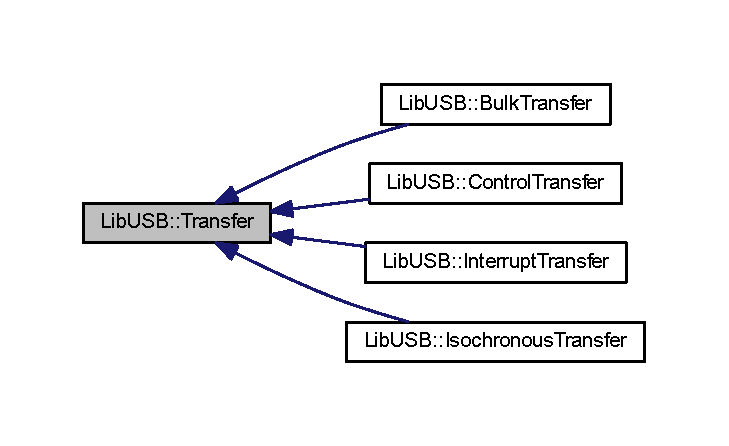
\includegraphics[width=350pt]{class_lib_u_s_b_1_1_transfer__inherit__graph}
\end{center}
\end{figure}
\subsection*{Public Member Functions}
\begin{DoxyCompactItemize}
\item 
\hypertarget{class_lib_u_s_b_1_1_transfer_afd32a556e274e2bb6eddb7d1490049dd}{\hyperlink{class_lib_u_s_b_1_1_transfer_afd32a556e274e2bb6eddb7d1490049dd}{Transfer} (std\-::shared\-\_\-ptr$<$ Transfer\-Impl $>$ p\-Transfer\-Impl)}\label{class_lib_u_s_b_1_1_transfer_afd32a556e274e2bb6eddb7d1490049dd}

\begin{DoxyCompactList}\small\item\em Constructor. \end{DoxyCompactList}\item 
\hypertarget{class_lib_u_s_b_1_1_transfer_ad34f40b2ff13df7906654211179e35be}{virtual \hyperlink{class_lib_u_s_b_1_1_transfer_ad34f40b2ff13df7906654211179e35be}{$\sim$\-Transfer} ()}\label{class_lib_u_s_b_1_1_transfer_ad34f40b2ff13df7906654211179e35be}

\begin{DoxyCompactList}\small\item\em Destructor. \end{DoxyCompactList}\item 
\hypertarget{class_lib_u_s_b_1_1_transfer_aecca9fae023e6c92b33c45e9918aad0a}{bool \hyperlink{class_lib_u_s_b_1_1_transfer_aecca9fae023e6c92b33c45e9918aad0a}{is\-Complete} ()}\label{class_lib_u_s_b_1_1_transfer_aecca9fae023e6c92b33c45e9918aad0a}

\begin{DoxyCompactList}\small\item\em Returns T\-R\-U\-E if the transfer is complete. \end{DoxyCompactList}\item 
\hypertarget{class_lib_u_s_b_1_1_transfer_a98e88da8dd01ae9686cc9b54eab17c65}{bool \hyperlink{class_lib_u_s_b_1_1_transfer_a98e88da8dd01ae9686cc9b54eab17c65}{is\-Successful} () const }\label{class_lib_u_s_b_1_1_transfer_a98e88da8dd01ae9686cc9b54eab17c65}

\begin{DoxyCompactList}\small\item\em Returns T\-R\-U\-E if the transfer is\-Successful. (\hyperlink{class_lib_u_s_b_1_1_transfer}{Transfer} M\-U\-S\-T be complete, throws any waiting exceptions) \end{DoxyCompactList}\item 
\hypertarget{class_lib_u_s_b_1_1_transfer_aaf7d05f7b96cb98fd201ec9266da2fb6}{void \hyperlink{class_lib_u_s_b_1_1_transfer_aaf7d05f7b96cb98fd201ec9266da2fb6}{set\-Transfer\-Buffer} (std\-::shared\-\_\-ptr$<$ unsigned char $>$ p\-Buffer, size\-\_\-t transfer\-Size)}\label{class_lib_u_s_b_1_1_transfer_aaf7d05f7b96cb98fd201ec9266da2fb6}

\begin{DoxyCompactList}\small\item\em Sets the amount of data to transfer in/out from the buffer. \end{DoxyCompactList}\item 
\hypertarget{class_lib_u_s_b_1_1_transfer_af8bab95cfa16ca472e67ece211c3ff6d}{std\-::shared\-\_\-ptr$<$ unsigned char $>$ \hyperlink{class_lib_u_s_b_1_1_transfer_af8bab95cfa16ca472e67ece211c3ff6d}{get\-Transfer\-Buffer} ()}\label{class_lib_u_s_b_1_1_transfer_af8bab95cfa16ca472e67ece211c3ff6d}

\begin{DoxyCompactList}\small\item\em Returns transfer buffer. \end{DoxyCompactList}\item 
\hypertarget{class_lib_u_s_b_1_1_transfer_a1de8c97baaa813aa076c8feff25c8010}{size\-\_\-t \hyperlink{class_lib_u_s_b_1_1_transfer_a1de8c97baaa813aa076c8feff25c8010}{Bytes\-Transferred} () const }\label{class_lib_u_s_b_1_1_transfer_a1de8c97baaa813aa076c8feff25c8010}

\begin{DoxyCompactList}\small\item\em Returns the amount of data written/read to/from the buffer. \end{DoxyCompactList}\item 
\hypertarget{class_lib_u_s_b_1_1_transfer_af1b7c2aca86e4fa5d781e375132d9e32}{void \hyperlink{class_lib_u_s_b_1_1_transfer_af1b7c2aca86e4fa5d781e375132d9e32}{Set\-Timeout} (std\-::chrono\-::milliseconds timeout)}\label{class_lib_u_s_b_1_1_transfer_af1b7c2aca86e4fa5d781e375132d9e32}

\begin{DoxyCompactList}\small\item\em Sets the timeout period for the transfer (0 denotes infinity) \end{DoxyCompactList}\item 
\hypertarget{class_lib_u_s_b_1_1_transfer_ae871f26d99baaa9ec639e17bb3fd3fa8}{virtual void \hyperlink{class_lib_u_s_b_1_1_transfer_ae871f26d99baaa9ec639e17bb3fd3fa8}{Start} ()}\label{class_lib_u_s_b_1_1_transfer_ae871f26d99baaa9ec639e17bb3fd3fa8}

\begin{DoxyCompactList}\small\item\em Starts the transfer. \end{DoxyCompactList}\item 
\hypertarget{class_lib_u_s_b_1_1_transfer_a25c88d0e7f825f47bffa545b3109fcb3}{void \hyperlink{class_lib_u_s_b_1_1_transfer_a25c88d0e7f825f47bffa545b3109fcb3}{Async\-Start} ()}\label{class_lib_u_s_b_1_1_transfer_a25c88d0e7f825f47bffa545b3109fcb3}

\begin{DoxyCompactList}\small\item\em Starts an asynchronous transfer. \end{DoxyCompactList}\item 
\hypertarget{class_lib_u_s_b_1_1_transfer_a625044102e97538726eccba59a41f6a6}{virtual void \hyperlink{class_lib_u_s_b_1_1_transfer_a625044102e97538726eccba59a41f6a6}{Cancel} ()}\label{class_lib_u_s_b_1_1_transfer_a625044102e97538726eccba59a41f6a6}

\begin{DoxyCompactList}\small\item\em Stops/\-Cancels the transfer. \end{DoxyCompactList}\item 
\hypertarget{class_lib_u_s_b_1_1_transfer_a2545527a281fb10a8474d46cd4575d42}{virtual void \hyperlink{class_lib_u_s_b_1_1_transfer_a2545527a281fb10a8474d46cd4575d42}{Reset} ()}\label{class_lib_u_s_b_1_1_transfer_a2545527a281fb10a8474d46cd4575d42}

\begin{DoxyCompactList}\small\item\em Resets the transfer to be used again. \end{DoxyCompactList}\item 
\hypertarget{class_lib_u_s_b_1_1_transfer_a499e1d2d8d76ba3a01c16007d5240d32}{Transfer\-Result\-\_\-t \hyperlink{class_lib_u_s_b_1_1_transfer_a499e1d2d8d76ba3a01c16007d5240d32}{Result} () const }\label{class_lib_u_s_b_1_1_transfer_a499e1d2d8d76ba3a01c16007d5240d32}

\begin{DoxyCompactList}\small\item\em Returns the result of the transfer. \end{DoxyCompactList}\item 
\hypertarget{class_lib_u_s_b_1_1_transfer_a0c3819a498e103f14997f1a87f69873d}{virtual void \hyperlink{class_lib_u_s_b_1_1_transfer_a0c3819a498e103f14997f1a87f69873d}{Init} ()}\label{class_lib_u_s_b_1_1_transfer_a0c3819a498e103f14997f1a87f69873d}

\begin{DoxyCompactList}\small\item\em Initializes the object after construction is completed. \end{DoxyCompactList}\item 
\hypertarget{class_lib_u_s_b_1_1_transfer_ac8ac10245a2bdd4c90495de86c7c1480}{bool \hyperlink{class_lib_u_s_b_1_1_transfer_ac8ac10245a2bdd4c90495de86c7c1480}{Wait\-For\-Completion} ()}\label{class_lib_u_s_b_1_1_transfer_ac8ac10245a2bdd4c90495de86c7c1480}

\begin{DoxyCompactList}\small\item\em Waits until the \hyperlink{class_lib_u_s_b_1_1_transfer}{Transfer} is complete. \end{DoxyCompactList}\end{DoxyCompactItemize}
\subsection*{Protected Attributes}
\begin{DoxyCompactItemize}
\item 
std\-::shared\-\_\-ptr$<$ Transfer\-Impl $>$ \hyperlink{class_lib_u_s_b_1_1_transfer_a09688b01c634cfdb522fb0c229da7308}{m\-\_\-p\-Transfer\-Impl}
\begin{DoxyCompactList}\small\item\em Resolves Completion. \end{DoxyCompactList}\item 
\hypertarget{class_lib_u_s_b_1_1_transfer_a5ea1bdbaa5248a43d4f7b053220677a4}{std\-::future$<$ std\-::shared\-\_\-ptr\\*
$<$ Lib\-U\-S\-B\-::\-Transfer\-Impl $>$ $>$ \hyperlink{class_lib_u_s_b_1_1_transfer_a5ea1bdbaa5248a43d4f7b053220677a4}{m\-\_\-\-Transfer\-Future}}\label{class_lib_u_s_b_1_1_transfer_a5ea1bdbaa5248a43d4f7b053220677a4}

\begin{DoxyCompactList}\small\item\em Result of the \hyperlink{class_lib_u_s_b_1_1_transfer}{Transfer} (Transfer\-Impl) \end{DoxyCompactList}\item 
\hypertarget{class_lib_u_s_b_1_1_transfer_a86498992dc1076d2d14ca8a646746059}{bool \hyperlink{class_lib_u_s_b_1_1_transfer_a86498992dc1076d2d14ca8a646746059}{m\-\_\-\-Asynchronous\-Transfer\-Pending}}\label{class_lib_u_s_b_1_1_transfer_a86498992dc1076d2d14ca8a646746059}

\begin{DoxyCompactList}\small\item\em Asynchronous \hyperlink{class_lib_u_s_b_1_1_transfer}{Transfer} Flag (true once the thread is started.) \end{DoxyCompactList}\item 
\hypertarget{class_lib_u_s_b_1_1_transfer_aa2690da75e400b433123340d3c160f0c}{std\-::shared\-\_\-ptr$<$ bool $>$ \hyperlink{class_lib_u_s_b_1_1_transfer_aa2690da75e400b433123340d3c160f0c}{m\-\_\-\-Transfer\-Thread\-Running}}\label{class_lib_u_s_b_1_1_transfer_aa2690da75e400b433123340d3c160f0c}

\begin{DoxyCompactList}\small\item\em Indicates that the asynchronous operation is still running. \end{DoxyCompactList}\end{DoxyCompactItemize}


\subsection{Detailed Description}
U\-S\-B Data transfer object. 

\subsection{Member Data Documentation}
\hypertarget{class_lib_u_s_b_1_1_transfer_a09688b01c634cfdb522fb0c229da7308}{\index{Lib\-U\-S\-B\-::\-Transfer@{Lib\-U\-S\-B\-::\-Transfer}!m\-\_\-p\-Transfer\-Impl@{m\-\_\-p\-Transfer\-Impl}}
\index{m\-\_\-p\-Transfer\-Impl@{m\-\_\-p\-Transfer\-Impl}!LibUSB::Transfer@{Lib\-U\-S\-B\-::\-Transfer}}
\subsubsection[{m\-\_\-p\-Transfer\-Impl}]{\setlength{\rightskip}{0pt plus 5cm}std\-::shared\-\_\-ptr$<$Transfer\-Impl$>$ Lib\-U\-S\-B\-::\-Transfer\-::m\-\_\-p\-Transfer\-Impl\hspace{0.3cm}{\ttfamily [protected]}}}\label{class_lib_u_s_b_1_1_transfer_a09688b01c634cfdb522fb0c229da7308}


Resolves Completion. 

\hyperlink{class_lib_u_s_b_1_1_transfer}{Transfer} Implementation 

The documentation for this class was generated from the following file\-:\begin{DoxyCompactItemize}
\item 
headers/Transfer.\-h\end{DoxyCompactItemize}

\printindex
\end{document}
